% Сборка из этой папки: xelatex persona-process.tex (два прогона)
% или tectonic persona-process.tex.
\documentclass[11pt,a4paper]{article}
\usepackage{fontspec}
\usepackage[russian]{babel}
\usepackage[a4paper,left=22mm,right=22mm,top=20mm,bottom=20mm,footskip=10mm]{geometry}
\usepackage{xcolor,graphicx,tabularx,booktabs,fancyhdr,hyperref}

\IfFontExistsTF{Arial}{\setmainfont{Arial}}{\setmainfont{DejaVu Sans}}
\IfFontExistsTF{Georgia}{\newfontfamily\displayfont{Georgia}}{\newfontfamily\displayfont{DejaVu Serif}}
\definecolor{ink}{HTML}{2F4156}
\definecolor{accent}{HTML}{3E6575}
\definecolor{sky}{HTML}{E8F0F5}
\definecolor{paper}{HTML}{F5EFEB}
\definecolor{line}{HTML}{C8D9E6}
\definecolor{muted}{HTML}{4F6474}
\definecolor{warm}{HTML}{71461D}
\definecolor{brandteal}{HTML}{567C8D}
\color{ink}
\graphicspath{{figures/}{../../../static/icons/}}
\setlength{\parindent}{0pt}
\setlength{\parskip}{6pt}
\linespread{1.06}
\setlength{\emergencystretch}{2em}
\setlength{\headheight}{14pt}
\setlength{\fboxsep}{10pt}
\renewcommand{\arraystretch}{1.26}
\raggedbottom
\hypersetup{
  unicode=true,
  colorlinks=true, linkcolor=accent, urlcolor=accent,
  pdftitle={persōna. Описание процесса создания},
  pdfsubject={Цифровой деканат будущего. Материалы для жюри},
  pdfauthor={Команда persōna},
  pdflang={ru-RU}
}
\pagestyle{fancy}
\fancyhf{}
\newcommand{\chapterlabel}{Процесс создания}
\fancyfoot[L]{\footnotesize\color{muted}persōna \enspace / \enspace \chapterlabel}
\fancyfoot[R]{\small\color{muted}\thepage}
\renewcommand{\headrulewidth}{0pt}
\renewcommand{\footrulewidth}{0.4pt}

\newcommand{\eyebrow}[1]{\textcolor{accent}{\small\bfseries #1}\par}
\newcommand{\display}[1]{{\displayfont\fontsize{28}{32}\selectfont #1\par}}
\newcommand{\pagehead}[3]{%
  \pdfbookmark[1]{#3}{#1}%
  \eyebrow{#2}\vspace{5pt}\display{#3}\vspace{7pt}}
\newcommand{\chapterhead}[3]{%
  \gdef\chapterlabel{#2}%
  \hypertarget{chapter-#1}{}\label{chapter-#1}%
  \pdfbookmark[0]{#2. #3}{#1}%
  \eyebrow{ГЛАВА #2 / 06}\vspace{5pt}\display{#3}\vspace{7pt}}
\newcommand{\tocrow}[3]{%
  \hyperlink{chapter-#1}{\textbf{#2}\enspace #3\hfill\pageref{chapter-#1}}\par\vspace{3pt}}
\newcommand{\minorhead}[1]{\vspace{3pt}{\large\bfseries #1\par}\vspace{1pt}}
\newcommand{\shade}[2][sky]{%
  \par\noindent\colorbox{#1}{\parbox{\dimexpr\linewidth-2\fboxsep\relax}{#2}}\par}
\newcommand{\captiontext}[2]{{\fontsize{9.3}{12}\selectfont\color{muted}\textbf{#1}\enspace #2\par}}
\newcommand{\evidence}[1]{\mbox{\hyperlink{sources}{\textcolor{accent}{\small[#1]}}}}
\newcommand{\repo}[1]{\textcolor{muted}{\footnotesize\nolinkurl{#1}}}
\newcolumntype{L}[1]{>{\raggedright\arraybackslash}p{#1}}
\newcolumntype{Y}{>{\raggedright\arraybackslash}X}

\begin{document}
\thispagestyle{empty}
\pdfbookmark[0]{Описание процесса создания}{cover}
\eyebrow{ЦИФРОВОЙ ДЕКАНАТ БУДУЩЕГО / ПРОЦЕСС СОЗДАНИЯ}
\vspace{10mm}
{\displayfont\fontsize{56}{60}\selectfont persōna\par}
\vspace{3mm}
{\displayfont\fontsize{23}{29}\selectfont У учёбы есть лицо. Твоё.\par}
\vspace{10mm}
\begin{minipage}[t]{.53\linewidth}\vspace{0pt}\raggedright
Расписание, результаты учёбы, документы и связь с деканатом в одном кабинете студента.

\vspace{8mm}
\eyebrow{ШЕСТЬ ГЛАВ ОТ ЗАДАЧИ ДО ПРОВЕРКИ}
\vspace{3mm}
\tocrow{problem}{01}{Проблема и решения}
\tocrow{tools}{02}{Инструменты и среда}
\tocrow{prompts}{03}{Задания и диалоги}
\tocrow{early}{04}{Визуальная история}
\tocrow{security}{05}{Вход и защита данных}
\tocrow{manual}{06}{Ручные этапы}

\vspace{8mm}
{\small\color{muted}Конкурсный прототип\par
Локальная демонстрационная версия\par
21 ноября 2026 года\par}
\end{minipage}\hfill
\begin{minipage}[t]{.39\linewidth}\vspace{0pt}
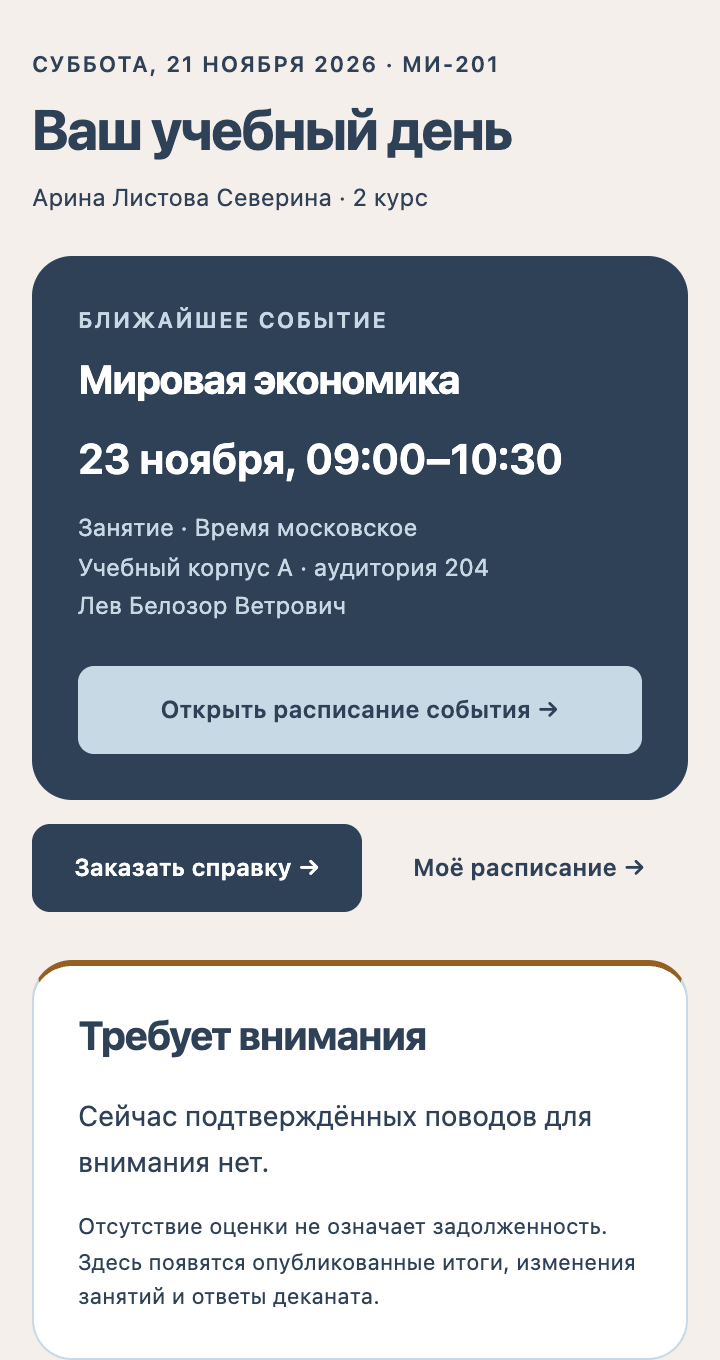
\includegraphics[width=\linewidth]{current-home.png}\par
\captiontext{Рабочая главная.}{Chrome, 360 px, 21 ноября.}
\end{minipage}
\vfill
\textcolor{line}{\rule{\linewidth}{0.6pt}}\par
{\small\color{muted}Все студенты, преподаватели и обращения на снимках вымышлены.}

\newpage
\chapterhead{problem}{01}{Проблема и решения}
Расписание на сайте, оценки в отдельной системе, справки через деканат, объявления в чатах: так описана исходная проблема конкурса. Мы связали её с конкретными действиями в кабинете. \evidence{1}

\vspace{4mm}
\begin{tabularx}{\linewidth}{@{}L{42mm}Y@{}}
\toprule
\textbf{Проблема студента} & \textbf{Решение и выбранные разделы}\\
\midrule
Нужно искать сведения в нескольких местах & \textbf{Главное и профиль.} Ближайшее событие после входа. ФИО, факультет, направление, курс и группа в одном профиле.\\[6pt]
Непонятно, куда идти после переноса & \textbf{Расписание.} День и неделя, пары сгруппированы по дням. «Было» и «Стало» показывают дату, время и аудиторию. Ссылка ведёт на новую дату.\\[6pt]
Трудно собрать картину учёбы & \textbf{Успеваемость и сессия.} Оценки и зачёты по дисциплинам, итог состояния учёбы и даты аттестации.\\[6pt]
Приходится уточнять готовность справки & \textbf{Заявки.} Отправка онлайн, статус, переписка и история в одной карточке. Оператор берёт заявку в работу и отвечает в ней.\\[6pt]
Изменения и сроки теряются в переписке & \textbf{Уведомления.} Объявления деканата и изменения с переходом к событию. \textbf{Личные дедлайны} дополняют ядро: студент задаёт срок и отмечает выполнение.\\
\bottomrule
\end{tabularx}

\vspace{7mm}
\shade[paper]{\textbf{Почему есть кабинет оператора.}\par
Он завершает сценарий справки: принимает обращение закреплённой группы, меняет статус и отвечает студенту. Результат виден в той же карточке после повторного входа. \evidence{4, 7}}

\vspace{6mm}
\minorhead{Что определило приоритеты}
Ближайшая пара и заметный перенос, понятный статус справки и связь с деканатом стали основой сценариев. Это исходные предположения команды. Три предоставленных текста ответов приведены далее целиком.

\hyperlink{survey-answers}{\textbf{Перейти к вопросам и ответам →}}

\newpage
\hypertarget{survey-answers}{}
\pagehead{survey}{01 \enspace / \enspace ПРОДУКТ}{Ответы на вопросы анкеты}
\vspace{4mm}
\shade[paper]{\textbf{1. Где вы в последний раз искали новое время или аудиторию пары?}\par\smallskip
«В последний раз, когда преподаватель внезапно перенес занятие, я сначала проверил закрепленное сообщение в общем чате группы — староста обычно оперативно пишет туда изменения. Убедившись, что там указана новая аудитория, я на всякий случай перепроверил информацию на официальном сайте вуза в разделе расписания, чтобы точно знать, в каком корпусе искать кабинет. Если бы в чате и на сайте данные разошлись, я бы написал старосте или заглянул в деканат.»}

\vspace{4mm}
\shade[paper]{\textbf{2. Как вы узнаёте, на каком этапе ваша заявка на справку?}\par\smallskip
«Обычно я подаю заявку через личный кабинет или пишу на официальную почту деканата. К сожалению, статус там обновляется не всегда, поэтому через пару дней я начинаю уточнять. Если справка нужна срочно (например, для банка или военкомата), я либо звоню секретарю напрямую, либо подхожу лично на перемене между парами. Иногда прошу куратора помочь узнать, готова ли бумага, если не получается дозвониться.»}

\vspace{4mm}
\shade[paper]{\textbf{3. Что вы открыли бы первым после входа в кабинет и почему?}\par\smallskip
«Первым делом я открываю расписание на сегодня и на завтра. Мне важно сразу увидеть не только время начала пар, но и номера корпусов, так как они находятся в разных частях города — от этого зависит, во сколько мне нужно выходить из дома. Кроме того, я сразу проверяю вкладку с уведомлениями от преподавателей, чтобы не пропустить внезапную отмену занятия или новое домашнее задание, которое нужно быстро распечатать.»}

\vspace{4mm}
\shade{\textbf{Что следует из этих ответов.}\par
Перенос должен показывать новое место без сверки нескольких каналов. Статус справки и ответ нужны в одной карточке. Расписание и изменения должны быть доступны сразу после входа.}

\newpage
\chapterhead{tools}{02}{Инструменты и среда}
\vspace{3mm}
\minorhead{Постановка, код и независимое ревью}
\textbf{OpenAI Codex и Codex CLI} — рабочий интерфейс и терминальная среда для архитектуры, кода, тестов, текстов и документации. Для планирования и постановки задач использовали \textbf{GPT-6.2 Sol / high}. Задачи реализовывали субагенты \textbf{GPT-6.2 Sol / low}.

\vspace{3mm}
\begin{tabularx}{\linewidth}{@{}L{37mm}Y@{}}
\toprule
\textbf{Роль} & \textbf{Инструменты и применение}\\
\midrule
Дизайн интерфейса & \textbf{Taste Skill.} Компоновка и ревью HTML-макетов и экранов: читаемость, отступы, фокус, размеры целей. Замечания чекера сопоставляли с поведением в браузере.\\[5pt]
Изображения & \textbf{OpenAI ImageGen.} Помощник, атлас поз, коты, аксессуары и обработка референса знака. \textbf{Python и Pillow} — подготовка PNG. \textbf{Canvas} — вывод и анимация игровых кадров.\\[5pt]
Документация & \textbf{OpenAI Docs и веб-поиск.} Первичные документы о настройках агентов и выбранных компонентах.\\[5pt]
Учебный чат & \textbf{OpenRouter / ERNIE Flash.} Живые проверки объяснения темы и отказов решать работу за студента.\\
\bottomrule
\end{tabularx}

\vspace{5mm}
\minorhead{Среда разработки, запуска и проверки}
{\small
\textbf{Приложение:} Python, Django, Django Templates, PostgreSQL, HTMX, собственные CSS и JavaScript.\par
\textbf{Запуск и история:} Bash, uv, Docker Compose, Git, GitHub. GitHub Actions настроен для проверок. Gunicorn, WhiteNoise и Caddy входят в схему выдачи приложения и статики.\par
\textbf{Проверки:} Ruff, pytest, Playwright, Chrome и Firefox. Браузерный осмотр дополняли серверными запросами и проверкой сохранения данных.}

\newpage
\chapterhead{prompts}{03}{Как ставили задачи ИИ}
\vspace{3mm}
\shade{\textbf{1. Доступ к профилю}\par\smallskip
Скрой каталог студентов в конкурсной версии. Если открыть чужую карточку по ссылке, покажи страницу 404. Проверь это под двумя тестовыми аккаунтами. Убедись, что каждый студент может открыть свой профиль.}
{\small\color{muted}Этап REL01. \evidence{7, 8}\par}

\vspace{4mm}
\shade{\textbf{2. Расписание и перенос пары}\par\smallskip
Собери пары одного дня в одну карточку. Покажи время, преподавателя и аудиторию. Для переноса сделай две части «Было» и «Стало» и добавь ссылку на новую дату. Проверь на телефоне и компьютере на примере переноса с 23 на 27 ноября.}
{\small\color{muted}Этапы U16 и U17. \evidence{4}\par}

\vspace{4mm}
\shade{\textbf{3. Заявка на справку}\par\smallskip
Добавь оператору кнопку «Принять в работу». Сделай так, чтобы студент и оператор могли писать друг другу в карточке заявки. Проверь, что ответ и статус «Готова» видны после повторного входа, а другой студент открыть заявку не может.}
{\small\color{muted}Этапы MSG01 и REQ01. \evidence{4, 7}\par}

\vspace{4mm}
\shade{\textbf{4. Буква P для логотипа}\par\smallskip
Возьми букву P из референса. Сохрани её форму и стеклянный блеск. Убери фон вокруг буквы и внутри неё, а блики подбери в цветах сайта. Сохрани результат как прозрачный PNG и проверь, различима ли буква в маленькой иконке.}
{\small\color{muted}Этапы U07 и CAT09. \evidence{10, 11}\par}

\vspace{3mm}
\minorhead{Как выглядела независимая проверка}
Исполнитель передавал фактический diff и результаты. Основной агент повторял ключевые шаги на изолированной PostgreSQL, сверял сохранение данных и возвращал точное замечание. Например, проверку мобильной карточки кота повторили после того, как в первой итерации на границе раскладок потерялась доступность звёзд. \evidence{6}

\newpage
\pagehead{ai-cases}{03 / ЗАДАНИЯ И ДИАЛОГИ}{Как уточняли результат}
\minorhead{AI07 / Учебная помощь без готовой работы}
Краткое изложение запроса и уточнения по журналу. \evidence{5}

\begin{tabularx}{\linewidth}{@{}L{31mm}Y@{}}
\textbf{Запрос} & Объяснять темы и методы. Отклонять просьбы выполнить тест, домашнее задание или экзамен за студента.\\[3pt]
\textbf{Первый ответ} & В живом прогоне модель отказалась решить активный экзамен, но повторила предложенные варианты ответа.\\[3pt]
\textbf{Уточнение} & Исправили серверную инструкцию: отказ не должен воспроизводить варианты экзамена.\\[3pt]
\textbf{Проверка} & Три корректных отказа и объяснение производной на четырёх вымышленных примерах. Поведение в любом другом диалоге зависит от модели.\\
\end{tabularx}

\vspace{5mm}
\begin{minipage}[t]{.59\linewidth}\vspace{0pt}
\minorhead{AI08 / Атлас помощника}
Попросили сохранить исходный портрет и положение тела, меняя только глаза, книгу и уши в четырёх клетках.

\shade{\eyebrow{ДОСЛОВНАЯ ВЫДЕРЖКА IMAGEGEN}
\small\raggedright\textit{“This is a registered animation contact sheet, not four reinterpretations, so all unchanged pixels especially body and head positions should align exactly.”}}

{\small В Chromium проверили четыре кадра, паузу и статичную позу при уменьшенном движении. \evidence{5}}
\end{minipage}\hfill
\begin{minipage}[t]{.35\linewidth}\vspace{0pt}

\includegraphics[width=\linewidth]{assistant-atlas.png}\par
\captiontext{Четыре состояния.}{Исходный атлас AI08, прозрачный PNG 1254 × 1254.}
\end{minipage}

\newpage
\chapterhead{early}{04}{От идеи к рабочему кабинету}
На этапе идеи в сценариях описали вход, ближайшую пару, оценки и путь заказа справки. Первую компоновку проверили как HTML-предпросмотр под рабочим названием «Кампус». Затем команда выбрала название persōna и палитру. \evidence{1, 3}

\vspace{3mm}
\begin{minipage}[t]{.46\linewidth}\vspace{0pt}
\centering
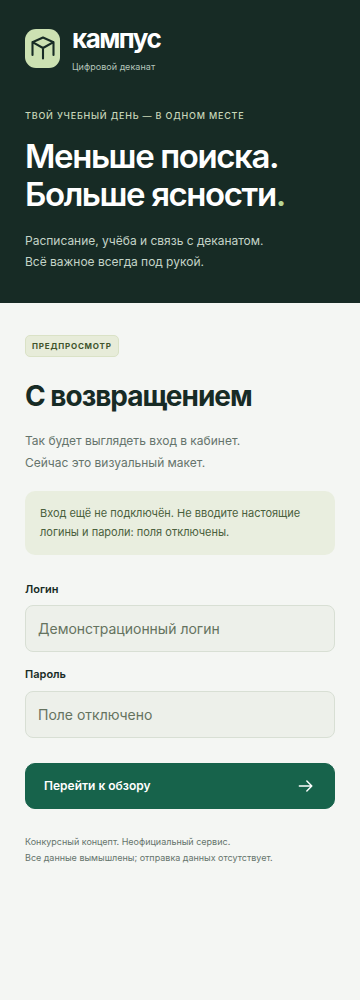
\includegraphics[height=151mm,width=\linewidth,keepaspectratio]{preview-login.png}\par
\raggedright\captiontext{01 \enspace Вход.}{В раннем макете логин и пароль отключены. На экране проверяли текст и компоновку.}
\end{minipage}\hfill
\begin{minipage}[t]{.46\linewidth}\vspace{0pt}
\centering
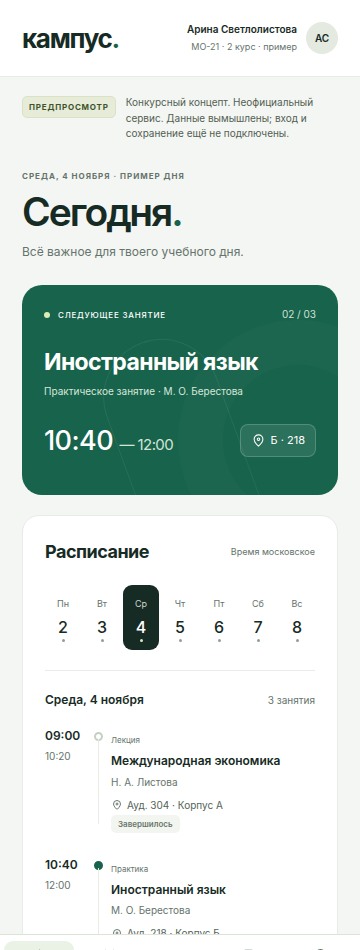
\includegraphics[height=151mm,width=\linewidth,keepaspectratio]{preview-home.png}\par
\raggedright\captiontext{02 \enspace Главная.}{Начало ранней страницы с ближайшей парой и планом недели.}
\end{minipage}

\vspace{2mm}
{\small\color{muted}Архивные снимки U02/F01, 4 ноября 2026 года, 360 px.}

\newpage
\pagehead{cat-design}{04 \enspace / \enspace СКРИНШОТЫ И ЭСКИЗЫ}{Как менялись коты}
Кот — персонаж короткой игры. Референс хромированного котёнка сменили пиксельные листы, затем генератор кадров на сетке 48 × 48. У Сони, Отличника и Маленького хаоса сохраняли общую позу и меняли мимику. \evidence{10}

\vspace{3mm}

\includegraphics[width=\linewidth]{cats-early.png}\par
\captiontext{Ранние спрайты из генератора.}{Слева направо Соня, Отличник и Маленький хаос. Общую форму различают мимика и очки. CAT07.}

\vspace{4mm}

\includegraphics[width=\linewidth]{cats-style.png}\par
\captiontext{Новая серия ImageGen.}{Те же три характера в палитре учебного помощника. Это мастер-иллюстрации для подготовки игровых кадров. CAT08.}

\vspace{4mm}
\begin{minipage}[t]{.47\linewidth}\vspace{0pt}

\includegraphics[width=\linewidth]{cat-animation-before.png}\par
\captiontext{До / CAT09.}{В удивлённой позе глаза стали прямоугольными.}
\end{minipage}\hfill
\begin{minipage}[t]{.47\linewidth}\vspace{0pt}

\includegraphics[width=\linewidth]{cat-animation-after.png}\par
\captiontext{После / CAT09.}{Вернули округлую форму зрачков и блик.}
\end{minipage}

\vspace{4mm}
\shade[paper]{\small\textbf{От картинки к движению.} Мастер-иллюстрации подготовили для Canvas на сетке 48 × 48. Тело, голова и хвост двигаются отдельно. После правок мимики, шеи и хвоста проверили геометрию 150 кадров и повторили 43 теста CAT09. \evidence{10}}

\newpage
\pagehead{brand-design}{04 \enspace / \enspace СКРИНШОТЫ И ЭСКИЗЫ}{Как появился знак persōna}
У первого макета «Кампус» рядом с названием стоял куб. После выбора названия persōna команда передала референсы буквы P и цветовой палитры. Так появилась задача сделать один знак для шапки, иконки вкладки и фона входа. \evidence{3, 11}

\vspace{4mm}
\begin{minipage}[t]{.43\linewidth}\vspace{0pt}
{\setlength{\fboxsep}{5pt}\colorbox{ink}{
\includegraphics[width=\dimexpr\linewidth-2\fboxsep\relax]{persona-mark.png}}}\par
\captiontext{Итоговая буква P.}{Прозрачный PNG 1254 × 1254 из проекта. Тёмная подложка добавлена при вёрстке отчёта.}
\end{minipage}\hfill
\begin{minipage}[t]{.51\linewidth}\vspace{0pt}\raggedright

\includegraphics[width=43mm]{brand-campus.png}\par
\captiontext{Ранний знак.}{Куб на экране входа «Кампуса». U02/F01.}
\vspace{4mm}
\minorhead{1. Задали форму и прозрачность}
В ImageGen передали референс и попросили сохранить каллиграфический силуэт P, острые засечки и стеклянные контуры. Участки вокруг буквы и внутри неё требовалось сделать прозрачными.
\end{minipage}

\vspace{5mm}
\minorhead{2. Перенесли отражения в палитру кабинета}
В промпте перечислили пять точных цветов для бликов и теней, чтобы буква сочеталась с фоном входа и навигацией. \evidence{11}

\vspace{2mm}
\begin{tabularx}{\linewidth}{@{}YYYYY@{}}
\textcolor{ink}{\rule{\linewidth}{13pt}} &
\textcolor{brandteal}{\rule{\linewidth}{13pt}} &
\textcolor{line}{\rule{\linewidth}{13pt}} &
\textcolor{paper}{\rule{\linewidth}{13pt}} &
{\setlength{\fboxsep}{0pt}\fcolorbox{line}{white}{\rule{\dimexpr\linewidth-2\fboxrule\relax}{0pt}\rule{0pt}{12.2pt}}}\\
{\small \#2F4156} & {\small \#567C8D} & {\small \#C8D9E6} & {\small \#F5EFEB} & {\small \#FFFFFF}\\
\end{tabularx}

\vspace{5mm}
\minorhead{3. Проверили два масштаба}
Крупный PNG использовали на экране входа. Позднее из того же рисунка экспортировали компактный PNG 96 × 96 для шапки и вкладки. При проверке на ширинах от 360 до 1440 px посмотрели загрузку знака, читаемость формы входа и доступность кнопки. \evidence{10, 11}

\vspace{4mm}
\shade[paper]{\textbf{Происхождение.} Форму буквы взяли из предоставленного референса. Разрешение на публичное распространение исходного рисунка и производных в журнале пока не подтверждено. \evidence{11}}

\newpage
\pagehead{iteration}{04 \enspace / \enspace СКРИНШОТЫ}{Что не сработало на телефоне}
При раскрытии карточки кота на 360 px она оказалась поверх формы учебного помощника. В браузере проверили, можно ли нажать поле и кнопку. \evidence{6}

\vspace{2mm}
\begin{minipage}[t]{.46\linewidth}\vspace{0pt}
\eyebrow{ДО ИСПРАВЛЕНИЯ}
\centering
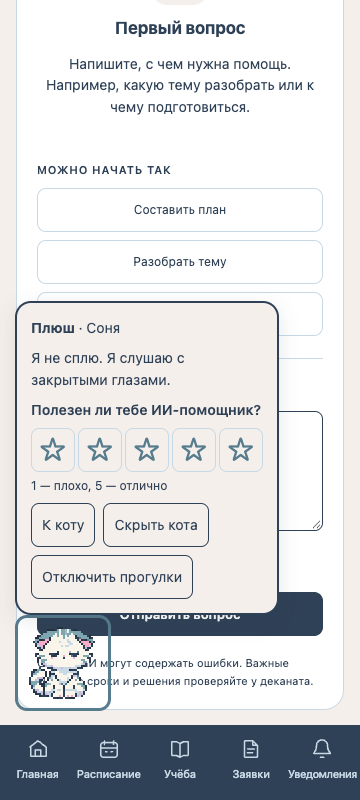
\includegraphics[height=147mm,width=\linewidth,keepaspectratio]{cat-before.png}\par
\raggedright\captiontext{03 \enspace Перекрытие.}{Открытая карточка лежит поверх области ввода и мешает отправке вопроса.}
\end{minipage}\hfill
\begin{minipage}[t]{.46\linewidth}\vspace{0pt}
\eyebrow{ПОСЛЕ ИСПРАВЛЕНИЯ}
\centering
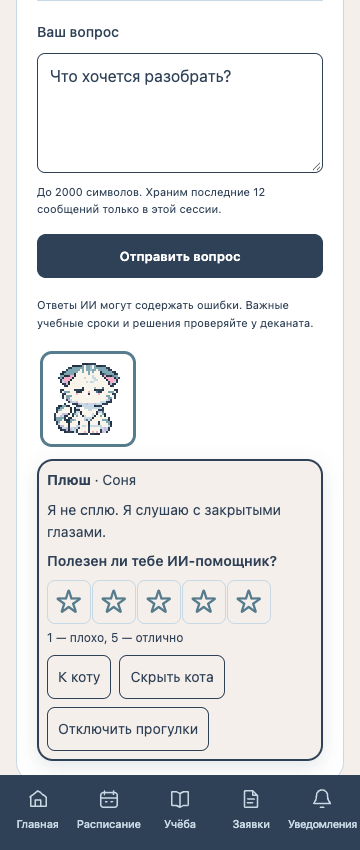
\includegraphics[height=147mm,width=\linewidth,keepaspectratio]{cat-after.png}\par
\raggedright\captiontext{04 \enspace Рабочая форма.}{Карточка расположена под формой. Вопрос и оценка котику доступны отдельно.}
\end{minipage}

\vspace{3mm}
\shade[paper]{\small\textbf{Повторная проверка.} В Chrome подтвердили доступность поля и отправки, фокус после смены ширины и запись оценки 4 из 5 в PostgreSQL. Снимки сделаны 20 ноября.}

\vspace{3mm}
{\small\color{muted}\textbf{Другие исправления.} Из теста чёткости исключили декоративный фон. Убрали 218 архивных файлов из выдаваемой статики и проверили 436 старых адресов на 404. Для переноса слогана расширили область до 176 px и повторили браузерную проверку. \evidence{12}}

\newpage
\pagehead{study}{04 / РАБОЧАЯ ВЕРСИЯ}{Расписание и успеваемость}
Главная с ближайшим событием показана на обложке. От неё студент переходит к занятиям и результатам учёбы. Ниже — локальные кадры с вымышленными данными. \evidence{4, 7}

\vspace{5mm}
\begin{minipage}[t]{.46\linewidth}\vspace{0pt}
\eyebrow{01 / ИЗМЕНЕНИЕ РАСПИСАНИЯ}
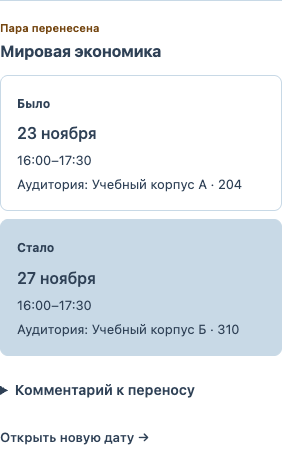
\includegraphics[width=\linewidth]{lesson-move.png}\par
\vspace{3mm}
\captiontext{Было → Стало.}{Дата, время и аудитория видны рядом. Ссылка открывает новую дату. U17, 20 ноября 2026 года, 360 px.}
\end{minipage}\hfill
\begin{minipage}[t]{.46\linewidth}\vspace{0pt}
\eyebrow{02 / ИТОГИ УЧЁБЫ}
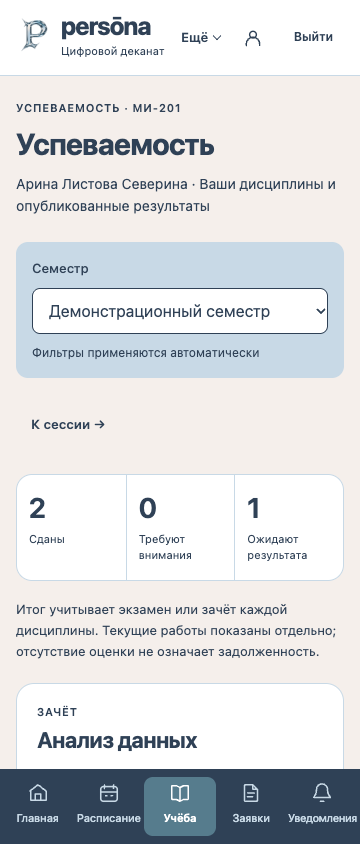
\includegraphics[width=\linewidth,height=165mm,keepaspectratio]{study-results-360.png}\par
\vspace{3mm}
\captiontext{Оценки и зачёты.}{Сводка сданных и ожидаемых результатов и начало списка дисциплин. REL09, 20 ноября 2026 года, 360 px.}
\end{minipage}

\vfill
\shade[paper]{\textbf{Один путь.} Вход → ближайшая пара → перенос или результаты → заявка. Данные привязаны к вошедшему студенту. Следующая страница показывает продолжение сценария у студента и оператора.}

\newpage
\pagehead{result}{04 / РАБОЧАЯ ВЕРСИЯ}{Справка: от заявки до ответа}
Студент отправляет заявку, оператор закреплённой группы принимает её в работу и отвечает. После повторного входа студент видит готовый результат в той же карточке. \evidence{4, 7}

\vspace{4mm}
\eyebrow{01 / ОПЕРАТОР ПРИНИМАЕТ ЗАЯВКУ}

\includegraphics[width=.85\linewidth]{current-operator-action.png}\par
\captiontext{Одно действие.}{Кнопка «Принять в работу» вместо списка переходов. Фрагмент экрана на 1440 px.}

\vspace{7mm}
\begin{minipage}[t]{.47\linewidth}\vspace{0pt}
\eyebrow{02 / СТУДЕНТ ВИДИТ РЕЗУЛЬТАТ}

\includegraphics[width=\linewidth]{current-ready-title.png}\par
\vspace{4mm}
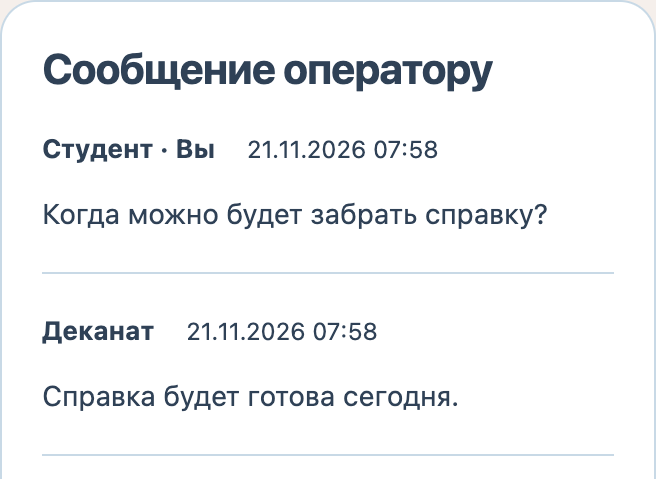
\includegraphics[width=\linewidth]{current-conversation.png}\par
\captiontext{Статус и ответ.}{«Готова» и сообщение оператора после повторной авторизации.}
\end{minipage}\hfill
\begin{minipage}[t]{.47\linewidth}\vspace{0pt}
\eyebrow{03 / ИСТОРИЯ СОХРАНЕНА}
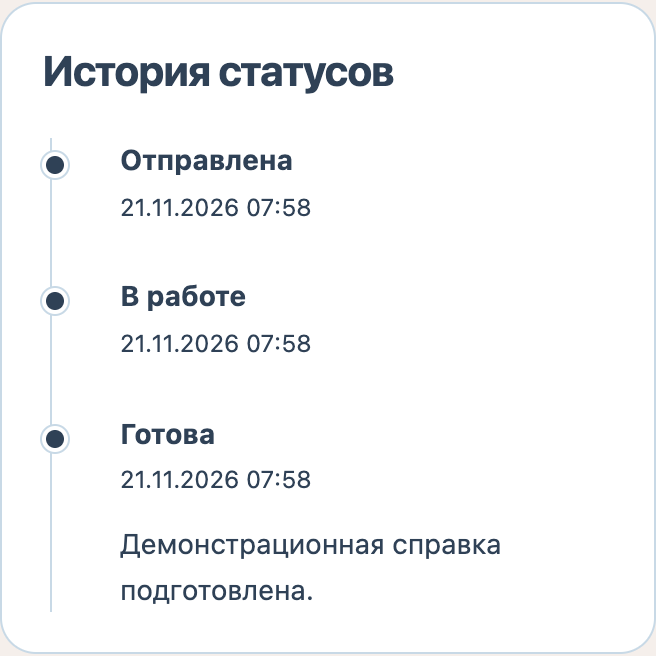
\includegraphics[width=\linewidth]{current-history.png}\par
\captiontext{Три события.}{История из той же заявки сохраняет ход обработки. Фрагмент экрана на 360 px.}
\end{minipage}

\vfill
{\small\color{muted}Снимки справки: локальный прогон 21 ноября 2026 года. Фрагменты обрезаны для читаемости. Кадры студента сняты на 360 px.}

\newpage
\chapterhead{security}{05}{Вход и защита данных}

Из браузера приходит запрос. Право читать или менять запись каждый раз проверяет сервер. Идентификатор записи в адресе сам по себе доступа не даёт. \evidence{8}

\vspace{5mm}
\begin{tabularx}{\linewidth}{@{}YYYY@{}}
\shade{\textbf{01}\par Вход} & \shade{\textbf{02}\par Сессия} & \shade{\textbf{03}\par Проверка прав} & \shade{\textbf{04}\par Свои данные}\\
\end{tabularx}
{\centering\color{accent}\textbf{Логин и пароль → сессия → права → свои данные}\par}

\vspace{6mm}
\minorhead{Пароль не хранится открытым}
Django сверяет пароль с хешем \textbf{Argon2}. После входа сервер создаёт сессию. Браузер получает её идентификатор в cookie с \textbf{HttpOnly}. Скрипты страницы не могут прочитать эту cookie.

\minorhead{Данные и история остаются в базе}
\textbf{PostgreSQL} хранит профили, расписание, результаты, заявки, сообщения и прочтение уведомлений. После проверки прав изменение записывается в базу. При смене статуса сохраняются переход и история, видимые после повторного входа.

\minorhead{Студент и оператор видят своё}
Студент получает свои записи, оператор — заявки закреплённых групп. Изменяющие формы защищены \textbf{CSRF}: сервер отклоняет попытку отправить форму с постороннего сайта. Ключ учебного чата задаётся в серверной конфигурации и не передаётся браузеру.

\vspace{6mm}
\shade[paper]{\eyebrow{ЛОКАЛЬНЫЙ ЭКСПЕРИМЕНТ / REL09 И REPORT01}
\textbf{Чужая ссылка → 404.} Во втором студенческом аккаунте чужие профиль и заявка недоступны. Повторный прогон 21 ноября также вернул 404 для чужой заявки.\par\smallskip
\textbf{Повторный вход → сохранённый результат.} Видны статус «Готова», ответ оператора и три события истории. \evidence{7}}

\vspace{4mm}
{\small\color{muted}Проверки проведены локально в браузере при 360 и 1440 px и серверными запросами. Работа опубликованного сайта и проверка на физическом телефоне здесь не подтверждаются.}

\newpage
\chapterhead{manual}{06}{Что сделали вручную}
По журналу и переписке подтверждаются следующие действия участников проекта. Браузерные и серверные прогоны, которые выполнял агент, в этот список не входят.

\begin{enumerate}
\setlength{\itemsep}{2pt}
\item Передали конкурсное задание и задали рабочий порядок. Разделили постановку, реализацию и приёмку, выбрали правило версионирования после проверки. \evidence{2}
\item Согласовали первый визуальный показ. Выбрали название persōna, предоставили референсы знака и палитры, уточнили расположение элементов фона. \evidence{3}
\item Запустили локальную установку и прислали журнал сбоя. Установка зависимостей прошла. Во время загрузки образа PostgreSQL истекло время TLS-соединения с Docker Hub, поэтому миграция не смогла подключиться к базе. \evidence{9}
\item Передали три текста ответов на вопросы анкеты для включения в отчёт. Размер выборки и порядок опроса не зафиксированы.
\item Уточнили интерфейс по видимым сценариям. Попросили сгруппировать пары по дням, переделать конкретный текст переноса, перенести переписку в заявку и заменить список действий при её принятии на кнопку. Выбрали слоган и его перенос на две строки. \evidence{4, 9}
\end{enumerate}

\vspace{5mm}
\hyperlink{appendix-tools}{\textbf{Инструменты и источники → приложение, стр. \pageref{appendix-tools}}}

\newpage
\gdef\chapterlabel{Приложение}
\hypertarget{appendix-tools}{}\label{appendix-tools}
\pdfbookmark[0]{Приложение. Инструменты и источники}{appendix}
\eyebrow{ПРИЛОЖЕНИЕ}\vspace{5pt}\display{Инструменты и источники}\vspace{5pt}
{\small
\textbf{OpenAI Codex и Codex CLI.} Рабочая среда для архитектуры, кода, тестов, текстов и документации.\par
\textbf{Taste Skill.} Компоновка и ревью HTML-макетов и экранов: читаемость, отступы, фокус и размеры целей.\par
\textbf{OpenAI ImageGen.} Помощник, атлас поз, коты, аксессуары и обработка референса знака. \textbf{Python и Pillow} — подготовка PNG. \textbf{Canvas} — вывод и анимация игровых кадров.\par
\textbf{OpenAI Docs и веб-поиск.} Первичные документы о настройках агентов и выбранных компонентах.\par
\textbf{OpenRouter / ERNIE Flash.} Учебный чат, живые проверки объяснения темы и отказов решать работу за студента.\par
\textbf{Стек.} Python, Django, Django Templates, PostgreSQL, HTMX, собственные CSS и JavaScript.\par
\textbf{Запуск и история.} Bash, uv, Docker Compose, Git, GitHub, GitHub Actions. Gunicorn, WhiteNoise и Caddy входят в схему выдачи приложения и статики.\par
\textbf{Проверки.} Ruff, pytest, Playwright, Chrome и Firefox. Браузерный осмотр, серверные запросы и проверка сохранения данных.}

\vspace{2mm}
\hypertarget{sources}{}
\minorhead{Где проверить материалы}
{\small Пути относятся к репозиторию. Ссылки [1–12] ведут сюда. Даты снимков указаны в подписях.}

{\fontsize{8.7}{11}\selectfont
\renewcommand{\arraystretch}{1.13}
\begin{tabularx}{\linewidth}{@{}L{7mm}Y@{}}
\toprule
\textbf{№} & \textbf{Источник в репозитории или журнале}\\
\midrule
1 & Требования конкурса и сценарии. \repo{README.md}, \repo{docs/product/scenarios.md}.\\
2 & Начальные настройки и постановки. \repo{docs/evidence/P00/prompt.md}, \repo{docs/agents/WORKFLOW.md}.\\
3 & Ранний макет и смена оформления. \repo{docs/evidence/U02-F01/review.md}, \repo{docs/evidence/U06/prompt.md}, \repo{docs/evidence/U13/review.md}.\\
4 & Доработки расписания и заявок. \repo{docs/evidence/U16/}, \repo{docs/evidence/U17/}, \repo{docs/evidence/MSG01/}, \repo{docs/evidence/REQ01/}, \repo{docs/evidence/ANN01/}.\\
5 & Провайдеры и графика. \repo{docs/evidence/AI03/}, \repo{docs/evidence/AI07/}, \repo{docs/evidence/AI08/imagegen.md}, \repo{docs/licenses.md}.\\
6 & Дефект, доработка и снимки. \repo{docs/evidence/REL08/review-02.md}.\\
7 & Сквозная репетиция и новые кадры. \repo{docs/evidence/REL09/review.md}, \repo{docs/evidence/REPORT01/review.md}.\\
8 & Архитектура, вход и защита. \repo{README.md}, \repo{docs/testing/security-review.md}, \repo{docs/evidence/REL01/review.md}.\\
9 & Диалог команды о локальном запуске и проверке статусов. \repo{docs/contest/report.md}, \repo{docs/evidence/COPY02/prompt.md}.\\
10 & Эскизы и анимация котов. \repo{docs/evidence/CAT01/}, \repo{docs/evidence/CAT02/}, \repo{docs/evidence/CAT05/}, \repo{docs/evidence/CAT07/}, \repo{docs/evidence/CAT08/}, \repo{docs/evidence/CAT09/}.\\
11 & Обработка буквы P и происхождение знака. \repo{docs/evidence/U07/imagegen.md}, \repo{docs/evidence/U07/review.md}, \repo{docs/evidence/REL10/review.md}.\\
12 & Исправление тестов, выдаваемой статики и переноса слогана. \repo{docs/evidence/REL02/review.md}, \repo{docs/evidence/REL11/review.md}, \repo{docs/evidence/COPY02/review.md}.\\
\bottomrule
\end{tabularx}}
\end{document}
